\chapter{Manipulación de bits}

Todos los datos en los programas de computadora se almacenan internamente como bits,
es decir, como números 0 y 1.
Este capítulo discute la representación en bits
de los enteros, y muestra ejemplos
de cómo usar las operaciones de bits.
Resulta que hay muchos usos para
la manipulación de bits en la programación de algoritmos.

\section{Representación en bits}

\index{representación en bits}

En programación, un entero de $n$ bits se almacena
internamente como un número binario que consta de $n$ bits.
Por ejemplo, el tipo \texttt{int} de C++ es
un tipo de 32 bits, lo que significa que cada número
\texttt{int} consta de 32 bits.

Aquí está la representación en bits del
número \texttt{int} 43:
\[00000000000000000000000000101011\]
Los bits de la representación se indexan de derecha a izquierda.
Para convertir una representación en bits $b_k \cdots b_2 b_1 b_0$ en un número,
podemos usar la fórmula
\[b_k 2^k + \ldots + b_2 2^2 + b_1 2^1 + b_0 2^0.\]
Por ejemplo,
\[1 \cdot 2^5 + 1 \cdot 2^3 + 1 \cdot 2^1 + 1 \cdot 2^0 = 43.\]

La representación en bits de un número es
\key{con signo} o \key{sin signo}.
Normalmente se usa una representación con signo,
lo que significa que pueden representarse tanto números
negativos como positivos.
Una variable con signo de $n$ bits puede contener cualquier
entero entre $-2^{n-1}$ y $2^{n-1}-1$.
Por ejemplo, el tipo \texttt{int} en C++ es
un tipo con signo, así que una variable \texttt{int} puede contener cualquier
entero entre $-2^{31}$ y $2^{31}-1$.

El primer bit en una representación con signo
es el signo del número (0 para números no negativos
y 1 para números negativos), y
los $n-1$ bits restantes contienen la magnitud del número.
Se usa el \key{complemento a dos}, lo que significa que el
número opuesto de un número se calcula primero
invirtiendo todos los bits del número,
y luego incrementando el número en uno.

Por ejemplo, la representación en bits del
número \texttt{int} $-43$ es
\[11111111111111111111111111010101.\]

En una representación sin signo, solo pueden usarse
números no negativos, pero la cota superior de los valores es mayor.
Una variable sin signo de $n$ bits puede contener cualquier
entero entre $0$ y $2^n-1$.
Por ejemplo, en C++, una variable \texttt{unsigned int}
puede contener cualquier entero entre $0$ y $2^{32}-1$.

Hay una conexión entre las
representaciones:
un número con signo $-x$ es igual a un número sin signo $2^n-x$.
Por ejemplo, el siguiente código muestra que
el número con signo $x=-43$ es igual al número
sin signo $y=2^{32}-43$:
\begin{lstlisting}
int x = -43;
unsigned int y = x;
cout << x << "\n"; // -43
cout << y << "\n"; // 4294967253
\end{lstlisting}

Si un número es mayor que la cota superior
de la representación en bits, el número se desbordará.
En una representación con signo,
el siguiente número después de $2^{n-1}-1$ es $-2^{n-1}$,
y en una representación sin signo,
el siguiente número después de $2^n-1$ es $0$.
Por ejemplo, considera el siguiente código:
\begin{lstlisting}
int x = 2147483647
cout << x << "\n"; // 2147483647
x++;
cout << x << "\n"; // -2147483648
\end{lstlisting}

Inicialmente, el valor de $x$ es $2^{31}-1$.
Este es el mayor valor que puede almacenarse
en una variable \texttt{int},
así que el siguiente número después de $2^{31}-1$ es $-2^{31}$.


\section{Operaciones de bits}

\newcommand\XOR{\mathbin{\char`\^}}

\subsubsection{Operación and}

\index{operación and}

La operación \key{and} $x$ \& $y$ produce un número
que tiene bits en uno en las posiciones donde tanto
$x$ como $y$ tienen bits en uno.
Por ejemplo, $22$ \& $26$ = 18, porque

\begin{center}
\begin{tabular}{rrr}
& 10110 & (22)\\
\& & 11010 & (26) \\
\hline
 = & 10010 & (18) \\
\end{tabular}
\end{center}

Usando la operación and, podemos comprobar si un número
$x$ es par porque
$x$ \& $1$ = 0 si $x$ es par, y
$x$ \& $1$ = 1 si $x$ es impar.
Más en general, $x$ es divisible entre $2^k$
exactamente cuando $x$ \& $(2^k-1)$ = 0.

\subsubsection{Operación or}

\index{operación or}

La operación \key{or} $x$ | $y$ produce un número
que tiene bits en uno en las posiciones donde al menos uno
de $x$ e $y$ tiene bits en uno.
Por ejemplo, $22$ | $26$ = 30, porque

\begin{center}
\begin{tabular}{rrr}
& 10110 & (22)\\
| & 11010 & (26) \\
\hline
 = & 11110 & (30) \\
\end{tabular}
\end{center}

\subsubsection{Operación xor}

\index{operación xor}

La operación \key{xor} $x$ $\XOR$ $y$ produce un número
que tiene bits en uno en las posiciones donde exactamente uno
de $x$ e $y$ tiene bits en uno.
Por ejemplo, $22$ $\XOR$ $26$ = 12, porque

\begin{center}
\begin{tabular}{rrr}
& 10110 & (22)\\
$\XOR$ & 11010 & (26) \\
\hline
 = & 01100 & (12) \\
\end{tabular}
\end{center}

\subsubsection{Operación not}

\index{operación not}

La operación \key{not} \textasciitilde$x$
produce un número donde todos los bits de $x$
han sido invertidos.
La fórmula \textasciitilde$x = -x-1$ se cumple,
por ejemplo, \textasciitilde$29 = -30$.

El resultado de la operación not a nivel de bits
depende de la longitud de la representación en bits,
porque la operación invierte todos los bits.
Por ejemplo, si los números son números \texttt{int}
de 32 bits, el resultado es el siguiente:

\begin{center}
\begin{tabular}{rrrr}
$x$ & = & 29 &   00000000000000000000000000011101 \\
\textasciitilde$x$ & = & $-30$ & 11111111111111111111111111100010 \\
\end{tabular}
\end{center}

\subsubsection{Desplazamientos de bits}

\index{desplazamiento de bits}

El desplazamiento de bits a la izquierda $x < < k$ agrega $k$
bits en cero al número,
y el desplazamiento de bits a la derecha $x > > k$
elimina los $k$ últimos bits del número.
Por ejemplo, $14 < < 2 = 56$,
porque $14$ y $56$ corresponden a 1110 y 111000.
De manera similar, $49 > > 3 = 6$,
porque $49$ y $6$ corresponden a 110001 y 110.

Nota que $x < < k$
corresponde a multiplicar $x$ por $2^k$,
y $x > > k$
corresponde a dividir $x$ entre $2^k$
redondeado hacia abajo a un entero.

\subsubsection{Aplicaciones}

Un número de la forma $1 < < k$ tiene un bit en uno
en la posición $k$ y todos los demás bits en cero,
así que podemos usar tales números para acceder a bits individuales de números.
En particular, el $k$-ésimo bit de un número está en uno
exactamente cuando $x$ \& $(1 < < k)$ no es cero.
El siguiente código imprime la representación en bits
de un número \texttt{int} $x$:

\begin{lstlisting}
for (int i = 31; i >= 0; i--) {
    if (x&(1<<i)) cout << "1";
    else cout << "0";
}
\end{lstlisting}

También es posible modificar bits individuales
de números usando ideas similares.
Por ejemplo, la fórmula $x$ | $(1 < < k)$
pone en uno el $k$-ésimo bit de $x$,
la fórmula
$x$ \& \textasciitilde $(1 < < k)$
pone en cero el $k$-ésimo bit de $x$,
y la fórmula
$x$ $\XOR$ $(1 < < k)$
invierte el $k$-ésimo bit de $x$.

La fórmula $x$ \& $(x-1)$ pone en cero el último
bit en uno de $x$,
y la fórmula $x$ \& $-x$ pone en cero todos los
bits en uno, excepto el último bit en uno.
La fórmula $x$ | $(x-1)$
invierte todos los bits después del último bit en uno.
Nota también que un número positivo $x$ es
una potencia de dos exactamente cuando $x$ \& $(x-1) = 0$.

\subsubsection*{Funciones adicionales}

El compilador g++ proporciona las siguientes
funciones para contar bits:

\begin{itemize}
\item
$\texttt{\_\_builtin\_clz}(x)$:
el número de ceros al principio del número
\item
$\texttt{\_\_builtin\_ctz}(x)$:
el número de ceros al final del número
\item
$\texttt{\_\_builtin\_popcount}(x)$:
el número de unos en el número
\item
$\texttt{\_\_builtin\_parity}(x)$:
la paridad (par o impar) del número de unos
\end{itemize}
\begin{samepage}

Las funciones pueden usarse de la siguiente manera:
\begin{lstlisting}
int x = 5328; // 00000000000000000001010011010000
cout << __builtin_clz(x) << "\n"; // 19
cout << __builtin_ctz(x) << "\n"; // 4
cout << __builtin_popcount(x) << "\n"; // 5
cout << __builtin_parity(x) << "\n"; // 1
\end{lstlisting}
\end{samepage}

Aunque las funciones anteriores solo admiten números \texttt{int},
también hay versiones \texttt{long long} de
las funciones disponibles con el sufijo \texttt{ll}.

\section{Representar conjuntos}

Todo subconjunto de un conjunto
$\{0,1,2,\ldots,n-1\}$
puede representarse como un entero de $n$ bits
cuyos bits en uno indican qué
elementos pertenecen al subconjunto.
Esta es una forma eficiente de representar conjuntos,
porque cada elemento requiere solo un bit de memoria,
y las operaciones de conjuntos pueden implementarse como operaciones de bits.

Por ejemplo, como \texttt{int} es un tipo de 32 bits,
un número \texttt{int} puede representar cualquier subconjunto
del conjunto $\{0,1,2,\ldots,31\}$.
La representación en bits del conjunto $\{1,3,4,8\}$ es
\[00000000000000000000000100011010,\]
que corresponde al número $2^8+2^4+2^3+2^1=282$.

\subsubsection{Implementación de conjuntos}

El siguiente código declara una variable
\texttt{int} $x$ que puede contener
un subconjunto de $\{0,1,2,\ldots,31\}$.
Después de esto, el código agrega los elementos 1, 3, 4 y 8
al conjunto e imprime el tamaño del conjunto.
\begin{lstlisting}
int x = 0;
x |= (1<<1);
x |= (1<<3);
x |= (1<<4);
x |= (1<<8);
cout << __builtin_popcount(x) << "\n"; // 4
\end{lstlisting}
Luego, el siguiente código imprime todos los
elementos que pertenecen al conjunto:
\begin{lstlisting}
for (int i = 0; i < 32; i++) {
    if (x&(1<<i)) cout << i << " ";
}
// output: 1 3 4 8
\end{lstlisting}

\subsubsection{Operaciones de conjuntos}

Las operaciones de conjuntos pueden implementarse de la siguiente manera como operaciones de bits:

\begin{center}
\begin{tabular}{lll}
& sintaxis de conjuntos & sintaxis de bits \\
\hline
intersección & $a \cap b$ & $a$ \& $b$ \\
unión & $a \cup b$ & $a$ | $b$ \\
complemento & $\bar a$ & \textasciitilde$a$ \\
diferencia & $a \setminus b$ & $a$ \& (\textasciitilde$b$) \\
\end{tabular}
\end{center}

Por ejemplo, el siguiente código primero construye
los conjuntos $x=\{1,3,4,8\}$ e $y=\{3,6,8,9\}$,
y luego construye el conjunto $z = x \cup y = \{1,3,4,6,8,9\}$:

\begin{lstlisting}
int x = (1<<1)|(1<<3)|(1<<4)|(1<<8);
int y = (1<<3)|(1<<6)|(1<<8)|(1<<9);
int z = x|y;
cout << __builtin_popcount(z) << "\n"; // 6
\end{lstlisting}

\subsubsection{Recorrer subconjuntos}

El siguiente código recorre
los subconjuntos de $\{0,1,\ldots,n-1\}$:

\begin{lstlisting}
for (int b = 0; b < (1<<n); b++) {
    // process subset b
}
\end{lstlisting}
El siguiente código recorre
los subconjuntos con exactamente $k$ elementos:
\begin{lstlisting}
for (int b = 0; b < (1<<n); b++) {
    if (__builtin_popcount(b) == k) {
        // process subset b
    }
}
\end{lstlisting}
El siguiente código recorre los subconjuntos
de un conjunto $x$:
\begin{lstlisting}
int b = 0;
do {
    // process subset b
} while (b=(b-x)&x);
\end{lstlisting}

\section{Optimizaciones con bits}

Muchos algoritmos pueden optimizarse usando
operaciones de bits.
Tales optimizaciones no cambian la
complejidad temporal del algoritmo,
pero pueden tener un gran impacto
en el tiempo de ejecución real del código.
En esta sección discutimos ejemplos
de tales situaciones.

\subsubsection{Distancias de Hamming}

\index{distancia de Hamming}
La \key{distancia de Hamming}
$\texttt{hamming}(a,b)$ entre dos
cadenas $a$ y $b$ de igual longitud es
el número de posiciones donde las cadenas difieren.
Por ejemplo,
\[\texttt{hamming}(01101,11001)=2.\]

Considera el siguiente problema: Dada
una lista de $n$ cadenas de bits, cada una de longitud $k$,
calcular la distancia de Hamming mínima
entre dos cadenas de la lista.
Por ejemplo, la respuesta para $[00111,01101,11110]$
es 2, porque
\begin{itemize}[noitemsep]
\item $\texttt{hamming}(00111,01101)=2$,
\item $\texttt{hamming}(00111,11110)=3$, y
\item $\texttt{hamming}(01101,11110)=3$.
\end{itemize}

Una forma directa de resolver el problema es
recorrer todos los pares de cadenas y calcular
sus distancias de Hamming,
lo que produce un algoritmo de tiempo $O(n^2 k)$.
La siguiente función puede usarse para
calcular distancias:
\begin{lstlisting}
int hamming(string a, string b) {
    int d = 0;
    for (int i = 0; i < k; i++) {
        if (a[i] != b[i]) d++;
    }
    return d;
}
\end{lstlisting}

Sin embargo, si $k$ es pequeño, podemos optimizar el código
almacenando las cadenas de bits como enteros y
calculando las distancias de Hamming usando operaciones de bits.
En particular, si $k \le 32$, podemos simplemente almacenar
las cadenas como valores \texttt{int} y usar la
siguiente función para calcular distancias:
\begin{lstlisting}
int hamming(int a, int b) {
    return __builtin_popcount(a^b);
}
\end{lstlisting}
En la función anterior, la operación xor construye
una cadena de bits que tiene bits en uno en las posiciones
donde $a$ y $b$ difieren.
Luego, el número de bits se calcula usando
la función \texttt{\_\_builtin\_popcount}.

Para comparar las implementaciones, generamos
una lista de 10000 cadenas de bits aleatorias de longitud 30.
Usando el primer enfoque, la búsqueda tomó
13.5 segundos, y después de la optimización con bits,
solo tomó 0.5 segundos.
Así, el código optimizado con bits fue casi
30 veces más rápido que el código original.

\subsubsection{Contar subcuadrículas}

Como otro ejemplo, considera el
siguiente problema:
Dada una cuadrícula de $n \times n$ donde
cada casilla es negra (1) o blanca (0),
calcular el número de subcuadrículas
cuyas cuatro esquinas son negras.
Por ejemplo, la cuadrícula
\begin{center}
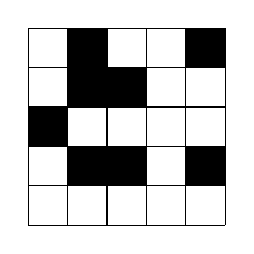
\begin{tikzpicture}[scale=0.5]
\fill[black] (1,1) rectangle (2,2);
\fill[black] (1,4) rectangle (2,5);
\fill[black] (4,1) rectangle (5,2);
\fill[black] (4,4) rectangle (5,5);
\fill[black] (1,3) rectangle (2,4);
\fill[black] (2,3) rectangle (3,4);
\fill[black] (2,1) rectangle (3,2);
\fill[black] (0,2) rectangle (1,3);
\draw (0,0) grid (5,5);
\end{tikzpicture}
\end{center}
contiene dos de tales subcuadrículas:
\begin{center}
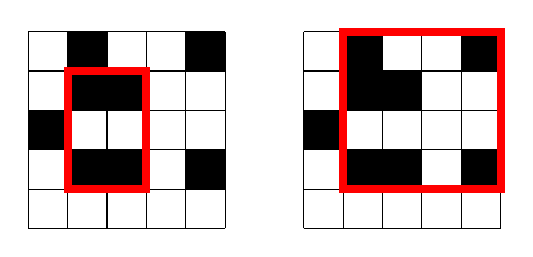
\begin{tikzpicture}[scale=0.5]
\fill[black] (1,1) rectangle (2,2);
\fill[black] (1,4) rectangle (2,5);
\fill[black] (4,1) rectangle (5,2);
\fill[black] (4,4) rectangle (5,5);
\fill[black] (1,3) rectangle (2,4);
\fill[black] (2,3) rectangle (3,4);
\fill[black] (2,1) rectangle (3,2);
\fill[black] (0,2) rectangle (1,3);
\draw (0,0) grid (5,5);

\fill[black] (7+1,1) rectangle (7+2,2);
\fill[black] (7+1,4) rectangle (7+2,5);
\fill[black] (7+4,1) rectangle (7+5,2);
\fill[black] (7+4,4) rectangle (7+5,5);
\fill[black] (7+1,3) rectangle (7+2,4);
\fill[black] (7+2,3) rectangle (7+3,4);
\fill[black] (7+2,1) rectangle (7+3,2);
\fill[black] (7+0,2) rectangle (7+1,3);
\draw (7+0,0) grid (7+5,5);

\draw[color=red,line width=1mm] (1,1) rectangle (3,4);
\draw[color=red,line width=1mm] (7+1,1) rectangle (7+5,5);
\end{tikzpicture}
\end{center}

Hay un algoritmo de tiempo $O(n^3)$ para resolver el problema:
recorrer todos los $O(n^2)$ pares de filas y para cada par
$(a,b)$ calcular el número de columnas que contienen una casilla negra
en ambas filas en tiempo $O(n)$.
El siguiente código supone que $\texttt{color}[y][x]$
denota el color en la fila $y$ y la columna $x$:
\begin{lstlisting}
int count = 0;
for (int i = 0; i < n; i++) {
    if (color[a][i] == 1 && color[b][i] == 1) count++;
}
\end{lstlisting}
Luego, esas columnas
representan $\texttt{count}(\texttt{count}-1)/2$ subcuadrículas con esquinas negras,
porque podemos elegir cualesquiera dos de ellas para formar una subcuadrícula.

Para optimizar este algoritmo, dividimos la cuadrícula en bloques
de columnas de modo que cada bloque conste de $N$
columnas consecutivas. Luego, cada fila se almacena como
una lista de números de $N$ bits que describen los colores
de las casillas. Ahora podemos procesar $N$ columnas al mismo tiempo
usando operaciones de bits. En el siguiente código,
$\texttt{color}[y][k]$ representa
un bloque de $N$ colores como bits.
\begin{lstlisting}
int count = 0;
for (int i = 0; i <= n/N; i++) {
    count += __builtin_popcount(color[a][i]&color[b][i]);
}
\end{lstlisting}
El algoritmo resultante funciona en tiempo $O(n^3/N)$.

Generamos una cuadrícula aleatoria de tamaño $2500 \times 2500$
y comparamos la implementación original y la optimizada con bits.
Mientras que el código original tomó $29.6$ segundos,
la versión optimizada con bits solo tomó $3.1$ segundos
con $N=32$ (números \texttt{int}) y $1.7$ segundos
con $N=64$ (números \texttt{long long}).

\section{Programación dinámica}

Las operaciones de bits ofrecen una forma eficiente y cómoda
de implementar algoritmos de programación dinámica
cuyos estados contienen subconjuntos de elementos,
porque tales estados pueden almacenarse como enteros.
A continuación discutimos ejemplos de combinar
operaciones de bits y programación dinámica.

\subsubsection{Selección óptima}

Como primer ejemplo, considera el siguiente problema:
Se nos dan los precios de $k$ productos
durante $n$ días, y queremos comprar cada producto
exactamente una vez.
Sin embargo, se nos permite comprar a lo sumo un producto
en un día.
¿Cuál es el precio total mínimo?
Por ejemplo, considera el siguiente escenario ($k=3$ y $n=8$):
\begin{center}
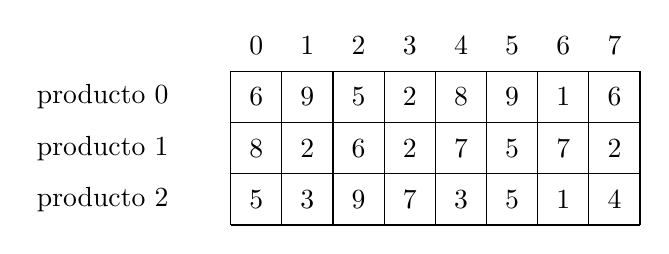
\begin{tikzpicture}[scale=.65]
    \draw (0, 0) grid (8,3);
    \node at (-2.5,2.5) {producto 0};
    \node at (-2.5,1.5) {producto 1};
    \node at (-2.5,0.5) {producto 2};

    \foreach \x in {0,...,7}
        {\node at (\x+0.5,3.5) {\x};}
    \foreach \x/\v in {0/6,1/9,2/5,3/2,4/8,5/9,6/1,7/6}
        {\node at (\x+0.5,2.5) {\v};}
    \foreach \x/\v in {0/8,1/2,2/6,3/2,4/7,5/5,6/7,7/2}
        {\node at (\x+0.5,1.5) {\v};}
    \foreach \x/\v in {0/5,1/3,2/9,3/7,4/3,5/5,6/1,7/4}
        {\node at (\x+0.5,0.5) {\v};}
\end{tikzpicture}
\end{center}
En este escenario, el precio total mínimo es $5$:
\begin{center}
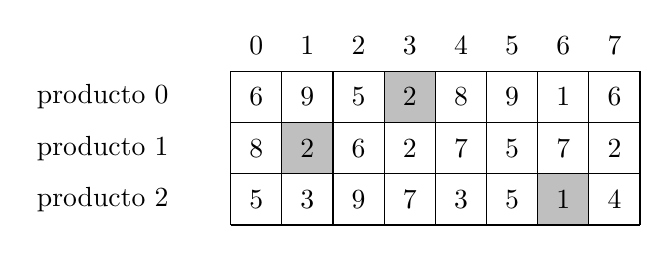
\begin{tikzpicture}[scale=.65]
    \fill [color=lightgray] (1, 1) rectangle (2, 2);
    \fill [color=lightgray] (3, 2) rectangle (4, 3);
    \fill [color=lightgray] (6, 0) rectangle (7, 1);
    \draw (0, 0) grid (8,3);
    \node at (-2.5,2.5) {producto 0};
    \node at (-2.5,1.5) {producto 1};
    \node at (-2.5,0.5) {producto 2};

    \foreach \x in {0,...,7}
        {\node at (\x+0.5,3.5) {\x};}
    \foreach \x/\v in {0/6,1/9,2/5,3/2,4/8,5/9,6/1,7/6}
        {\node at (\x+0.5,2.5) {\v};}
    \foreach \x/\v in {0/8,1/2,2/6,3/2,4/7,5/5,6/7,7/2}
        {\node at (\x+0.5,1.5) {\v};}
    \foreach \x/\v in {0/5,1/3,2/9,3/7,4/3,5/5,6/1,7/4}
        {\node at (\x+0.5,0.5) {\v};}
\end{tikzpicture}
\end{center}

Sea $\texttt{price}[x][d]$ el precio del producto $x$
en el día $d$.
Por ejemplo, en el escenario anterior $\texttt{price}[2][3] = 7$.
Luego, sea $\texttt{total}(S,d)$ el precio total mínimo
para comprar un subconjunto $S$ de productos para el día $d$.
Usando esta función, la solución al problema es
$\texttt{total}(\{0 \ldots k-1\},n-1)$.

Primero, $\texttt{total}(\emptyset,d) = 0$,
porque no cuesta nada comprar un conjunto vacío,
y $\texttt{total}(\{x\},0) = \texttt{price}[x][0]$,
porque hay una forma de comprar un producto el primer día.
Luego, puede usarse la siguiente recurrencia:
\begin{equation*}
\begin{split}
\texttt{total}(S,d) = \min( & \texttt{total}(S,d-1), \\
& \min_{x \in S} (\texttt{total}(S \setminus x,d-1)+\texttt{price}[x][d]))
\end{split}
\end{equation*}
Esto significa que o bien no compramos ningún producto el día $d$
o compramos un producto $x$ que pertenece a $S$.
En el último caso, eliminamos $x$ de $S$ y agregamos el
precio de $x$ al precio total.

El siguiente paso es calcular los valores de la función
usando programación dinámica.
Para almacenar los valores de la función, declaramos un arreglo
\begin{lstlisting}
int total[1<<K][N];
\end{lstlisting}
donde $K$ y $N$ son constantes suficientemente grandes.
La primera dimensión del arreglo corresponde a una
representación en bits de un subconjunto.

Primero, los casos donde $d=0$ pueden procesarse de la siguiente manera:
\begin{lstlisting}
for (int x = 0; x < k; x++) {
    total[1<<x][0] = price[x][0];
}
\end{lstlisting}
Luego, la recurrencia se traduce en el siguiente código:
\begin{lstlisting}
for (int d = 1; d < n; d++) {
    for (int s = 0; s < (1<<k); s++) {
        total[s][d] = total[s][d-1];
        for (int x = 0; x < k; x++) {
            if (s&(1<<x)) {
                total[s][d] = min(total[s][d],
                                    total[s^(1<<x)][d-1]+price[x][d]);
            }
        }
    }
}
\end{lstlisting}
La complejidad temporal del algoritmo es $O(n 2^k k)$.

\subsubsection{De permutaciones a subconjuntos}

Usando programación dinámica, a menudo es posible
cambiar una iteración sobre permutaciones por
una iteración sobre subconjuntos\footnote{Esta técnica fue introducida en 1962
por M. Held y R. M. Karp \cite{hel62}.}.
El beneficio de esto es que
$n!$, el número de permutaciones,
es mucho mayor que $2^n$, el número de subconjuntos.
Por ejemplo, si $n=20$, entonces
$n! \approx 2.4 \cdot 10^{18}$ y $2^n \approx 10^6$.
Así, para ciertos valores de $n$,
podemos recorrer eficientemente los subconjuntos pero no las permutaciones.

Como ejemplo, considera el siguiente problema:
Hay un ascensor con peso máximo $x$,
y $n$ personas con pesos conocidos
que quieren ir de la planta baja
al último piso.
¿Cuál es el número mínimo de viajes necesarios
si las personas entran al ascensor en un orden óptimo?

Por ejemplo, supongamos que $x=10$, $n=5$
y los pesos son los siguientes:
\begin{center}
\begin{tabular}{ll}
persona & peso \\
\hline
0 & 2 \\
1 & 3 \\
2 & 3 \\
3 & 5 \\
4 & 6 \\
\end{tabular}
\end{center}
En este caso, el número mínimo de viajes es 2.
Un orden óptimo es $\{0,2,3,1,4\}$,
que reparte a las personas en dos viajes:
primero $\{0,2,3\}$ (peso total 10),
y luego $\{1,4\}$ (peso total 9).

El problema puede resolverse fácilmente en tiempo $O(n! n)$
probando todas las permutaciones posibles de $n$ personas.
Sin embargo, podemos usar programación dinámica para obtener
un algoritmo más eficiente de tiempo $O(2^n n)$.
La idea es calcular para cada subconjunto de personas
dos valores: el número mínimo de viajes necesarios y
el peso mínimo de las personas que viajan en el último grupo.

Sea $\texttt{weight}[p]$ el peso de
la persona $p$.
Definimos dos funciones:
$\texttt{rides}(S)$ es el número mínimo de
viajes para un subconjunto $S$,
y $\texttt{last}(S)$ es el peso mínimo
del último viaje.
Por ejemplo, en el escenario anterior
\[ \texttt{rides}(\{1,3,4\})=2 \hspace{10px} \textrm{y}
\hspace{10px} \texttt{last}(\{1,3,4\})=5,\]
porque los viajes óptimos son $\{1,4\}$ y $\{3\}$,
y el segundo viaje tiene peso 5.
Por supuesto, nuestro objetivo final es calcular el valor
de $\texttt{rides}(\{0 \ldots n-1\})$.

Podemos calcular los valores
de las funciones recursivamente y luego aplicar
programación dinámica.
La idea es recorrer todas las personas
que pertenecen a $S$ y elegir de forma óptima
la última persona $p$ que entra al ascensor.
Cada una de tales elecciones produce un subproblema
para un subconjunto más pequeño de personas.
Si $\texttt{last}(S \setminus p)+\texttt{weight}[p] \le x$,
podemos agregar $p$ al último viaje.
En caso contrario, tenemos que reservar un nuevo viaje
que inicialmente solo contiene a $p$.

Para implementar la programación dinámica,
declaramos un arreglo
\begin{lstlisting}
pair<int,int> best[1<<N];
\end{lstlisting}
que contiene para cada subconjunto $S$
un par $(\texttt{rides}(S),\texttt{last}(S))$.
Establecemos el valor para un grupo vacío de la siguiente manera:
\begin{lstlisting}
best[0] = {1,0};
\end{lstlisting}
Luego, podemos llenar el arreglo de la siguiente manera:

\begin{lstlisting}
for (int s = 1; s < (1<<n); s++) {
    // initial value: n+1 rides are needed
    best[s] = {n+1,0};
    for (int p = 0; p < n; p++) {
        if (s&(1<<p)) {
            auto option = best[s^(1<<p)];
            if (option.second+weight[p] <= x) {
                // add p to an existing ride
                option.second += weight[p];
            } else {
                // reserve a new ride for p
                option.first++;
                option.second = weight[p];
            }
            best[s] = min(best[s], option);
        }
    }
}
\end{lstlisting}
Nota que el bucle anterior garantiza que
para cualesquiera dos subconjuntos $S_1$ y $S_2$
tales que $S_1 \subset S_2$, procesamos $S_1$ antes que $S_2$.
Así, los valores de programación dinámica se calculan en el
orden correcto.

\subsubsection{Contar subconjuntos}

Nuestro último problema de este capítulo es el siguiente:
Sea $X=\{0 \ldots n-1\}$, y a cada subconjunto $S \subset X$
se le asigna un entero $\texttt{value}[S]$.
Nuestra tarea es calcular para cada $S$
\[\texttt{sum}(S) = \sum_{A \subset S} \texttt{value}[A],\]
es decir, la suma de los valores de los subconjuntos de $S$.

Por ejemplo, supongamos que $n=3$ y los valores son los siguientes:
\begin{multicols}{2}
\begin{itemize}
\item $\texttt{value}[\emptyset] = 3$
\item $\texttt{value}[\{0\}] = 1$
\item $\texttt{value}[\{1\}] = 4$
\item $\texttt{value}[\{0,1\}] = 5$
\item $\texttt{value}[\{2\}] = 5$
\item $\texttt{value}[\{0,2\}] = 1$
\item $\texttt{value}[\{1,2\}] = 3$
\item $\texttt{value}[\{0,1,2\}] = 3$
\end{itemize}
\end{multicols}
En este caso, por ejemplo,
\begin{equation*}
\begin{split}
\texttt{sum}(\{0,2\}) &= \texttt{value}[\emptyset]+\texttt{value}[\{0\}]+\texttt{value}[\{2\}]+\texttt{value}[\{0,2\}] \\
                      &= 3 + 1 + 5 + 1 = 10.
\end{split}
\end{equation*}

Como hay un total de $2^n$ subconjuntos,
una posible solución es recorrer todos los
pares de subconjuntos en tiempo $O(2^{2n})$.
Sin embargo, usando programación dinámica, podemos
resolver el problema en tiempo $O(2^n n)$.
La idea es centrarnos en sumas donde los
elementos que pueden eliminarse de $S$ están restringidos.

Sea $\texttt{partial}(S,k)$ la suma de los
valores de los subconjuntos de $S$ con la restricción
de que solo los elementos $0 \ldots k$
pueden eliminarse de $S$.
Por ejemplo,
\[\texttt{partial}(\{0,2\},1)=\texttt{value}[\{2\}]+\texttt{value}[\{0,2\}],\]
porque solo podemos eliminar los elementos $0 \ldots 1$.
Podemos calcular los valores de \texttt{sum} usando
los valores de \texttt{partial}, porque
\[\texttt{sum}(S) = \texttt{partial}(S,n-1).\]
Los casos base de la función son
\[\texttt{partial}(S,-1)=\texttt{value}[S],\]
porque en este caso no puede eliminarse ningún elemento de $S$.
Luego, en el caso general podemos usar la siguiente recurrencia:
\begin{equation*}
    \texttt{partial}(S,k) = \begin{cases}
               \texttt{partial}(S,k-1) & k \notin S \\
               \texttt{partial}(S,k-1) + \texttt{partial}(S \setminus \{k\},k-1) & k \in S
           \end{cases}
\end{equation*}
Aquí nos centramos en el elemento $k$.
Si $k \in S$, tenemos dos opciones: podemos mantener $k$ en $S$
o eliminarlo de $S$.

Hay una forma particularmente ingeniosa de implementar el
cálculo de las sumas. Podemos declarar un arreglo
\begin{lstlisting}
int sum[1<<N];
\end{lstlisting}
que contendrá la suma de cada subconjunto.
El arreglo se inicializa de la siguiente manera:
\begin{lstlisting}
for (int s = 0; s < (1<<n); s++) {
    sum[s] = value[s];
}
\end{lstlisting}
Luego, podemos llenar el arreglo de la siguiente manera:
\begin{lstlisting}
for (int k = 0; k < n; k++) {
    for (int s = 0; s < (1<<n); s++) {
        if (s&(1<<k)) sum[s] += sum[s^(1<<k)];
    }
}
\end{lstlisting}
Este código calcula los valores de $\texttt{partial}(S,k)$
para $k=0 \ldots n-1$ en el arreglo \texttt{sum}.
Como $\texttt{partial}(S,k)$ siempre se basa en
$\texttt{partial}(S,k-1)$, podemos reutilizar el arreglo
\texttt{sum}, lo que produce una implementación muy eficiente.
